\begin{song}{title=\centering Nagasaki Hirošima \\\normalsize Mňága \&  Žďorp  \vspace*{-0.3cm}}  %% sem se napíše jméno songu a autor
\moveright 4.5cm \vbox{      %Varianta č. 1  ---> Jeden sloupec zarovnaný na střed	

\sloka
	^{C}Tramvají ^{G}dvojkou ^{F}jezdíval jsem ^{G}do ^{C}Židenic, ^{G\,F\,G}

	z ^{C}tak velký ^{G}lásky ^{F}většinou ^{G}nezbyde ^{Ami}nic.

	Z ^{F}takový ^{C}lásky ^{F}jsou kruhy ^{C}pod ^{G}očima

	a dvě ^{C}spálený ^{G}srdce -- ^{F}Nagasaki ^{G}Hirošima. ^{C\,G\,F\,G}

\sloka
	Jsou jistý věci co bych tesal do kamene,
	
	tam kde je láska tam je všechno dovolené
	
	a tam, kde není, tam mě to nezajímá.
	
	Jó dvě spálený srdce Nagasaki Hirošima.

\sloka
	Já nejsem svatej ani ty nejsi svatá,
	
	jablka z ráje bejvala jedovatá,
	
	jenže hezky jsi hřála, když mi někdy byla zima.
	
	Jó dvě spálený srdce Nagasaki Hirošima.

\sloka
	Tramvají dvojkou jezdíval jsem do Židenic,
	
	z takový lásky většinou nezbyde nic.
	
	Z takový lásky jsou kruhy pod očima

	/: a dvě spálený srdce Nagasaki Hirošma. :/
	
	/: A dvě spálený srdce Nagasaki Hirošma. :/


}
\setcounter{Slokočet}{0}
\end{song}


\begin{figure}[h]
\centering
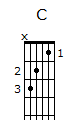
\includegraphics[scale=1.5]{../Akordy/c.png}
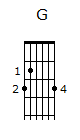
\includegraphics[scale=1.5]{../Akordy/g.png}
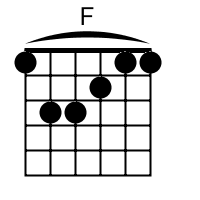
\includegraphics[scale=1.5]{../Akordy/f.png}
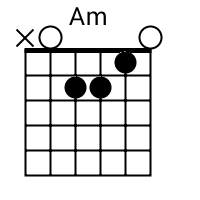
\includegraphics[scale=1.5]{../Akordy/am.png}
\end{figure}
